%\documentclass{...}

%modification history
% 9 jul 2011
% 29 nov 2011

\documentclass[11pt, letterpaper]{article}
\usepackage[margin=1in]{geometry}

% \documentclass[11pt, letterpaper]{article}
%
% % ----- margins -----
%
% \topmargin -1.5cm         % read Lamport p.163
% \oddsidemargin -0.04cm    % read Lamport p.163
% \evensidemargin -0.04cm   % same as oddsidemargin but for left-hand pages
%
% % ----- texts -----
%
% \textwidth 16.59cm
% \textheight 21.94cm
%
% % ----- indendts and spacing -----
%
% \parskip 0pt            	% spacing between paragraphs
% %\renewcommand{\baselinestretch}{1.5}	% uncomment for 1.5 spacing
%
% \parindent 7mm		      % leading space for paragraphs between lines
%
% % ----- page # -----
%
% %\pagestyle{empty}         % uncomment if don't want page numbers





\usepackage{amsfonts, amsmath, amssymb, amsthm}
\usepackage{comment}
\usepackage{graphicx}
\usepackage{ifthen}
\usepackage{latexsym}
%\usepackage{times}



%=== use the these packages if they are not already in use ===
\usepackage{amsfonts, amsmath, amssymb, amsthm}
\usepackage[nocompress]{cite}
\usepackage{color}
\usepackage{graphicx}
\usepackage{microtype}
\usepackage[normalem]{ulem}
\usepackage{wrapfig}
%=============================================================

%===== fonts =====
\def\ttt{\texttt}
\def\tsc{\textsc}

%===== spacing =====

\def\extraspacing{\vspace{3mm} \noindent}
\def\figcapup{\vspace{-1mm}}
\def\figcapdown{\vspace{-0mm}}
\def\hgap{\textrm{\hspace{1mm}}}
\def\thmvgap{\vspace{0mm}}
\def\vgap{\vspace{1mm}}


%===== tabbing =====

\def\tab{\hspace{3mm}}
\def\tabpos{\hspace{4mm} \= \hspace{4mm} \= \hspace{4mm} \= \hspace{4mm} \=
\hspace{4mm} \= \hspace{4mm} \= \hspace{4mm} \= \hspace{4mm} \= \hspace{4mm}
\kill}
\newcommand{\mytab}[1]{\begin{tabbing}\tabpos #1\end{tabbing}}

%===== blocks =====

\newtheorem{theorem}{Theorem}
\newtheorem{lemma}{Lemma}
\newtheorem{corollary}{Corollary}
\newtheorem{proposition}{Proposition}
\newtheorem{definition}{Definition}
\newtheorem{problem}{Problem}

\newcommand{\boxminipg}[2]{\begin{center}\fbox{\begin{minipage}{#1}#2\end{minipage}}\end{center}}
\newcommand{\minipg}[2]{\begin{center}\begin{minipage}{#1}#2\end{minipage}\end{center}}
\newcommand{\myitems}[1]{\begin{itemize}#1\end{itemize}}
\newcommand{\myenums}[1]{\begin{enumerate}#1\end{enumerate}}
\newcommand{\myfig}[1]{\begin{figure}\centering #1\end{figure}}
\newcommand{\myfigstar}[1]{\begin{figure*}\centering #1\end{figure*}}

%===== math macros =====

\newcommand{\bm}[1]{\textrm{\boldmath${#1}$}}
% \newcommand{\smat}[2]{\left[\begin{tabular}{#1}#2\end{tabular}\right]}
% \newcommand{\bmat}[2]{\left|\begin{tabular}{#1}#2\end{tabular}\right|}
\newcommand{\bmat}[1]{\begin{bmatrix}#1\end{bmatrix}}
\newcommand{\vmat}[1]{\begin{vmatrix}#1\end{vmatrix}}
\newcommand{\myeqn}[1]{\begin{eqnarray}#1\end{eqnarray}}

\newcommand{\myset}[1]{\{#1\}}

%\def\bm{\boldmath}
%\def\defeq{\stackrel{\textrm{\tiny{def}}}{=}}
\def\mit{\mathit}
\def\defeq{:=}
\def\eps{\epsilon}
\def\fr{\frac}
\def\-{\mbox{-}}
\def\real{\mathbb{R}}

\def\tO{\tilde{O}}

\def\lc{\lceil}
\def\lf{\lfloor}
\def\rc{\rceil}
\def\rf{\rfloor}

\def\nn{\nonumber}

\def\Pr{\mathbf{Pr}}
\def\expt{\mathbf{E}}
\def\var{\mathbf{var}}

\def\dcl{\{\!\!\{}
\def\dcr{\}\!\!\}}
\def\bigdcl{\Big\{\!\!\Big\{}
\def\bigdcr{\Big\}\!\!\Big\}}
\def\bigmid{\textrm{ $\Big|$ }}

\def\*{\star}

\DeclareMathOperator*{\argmin}{arg\,min}
\DeclareMathOperator*{\polylg}{polylg}
\DeclareMathOperator*{\polylog}{polylog}
\DeclareMathOperator*{\intr}{\cap}


%===== misc =====

\def\done{\qed \vspace{2mm}}	% end of proof
\def\tbc{\hspace*{\fill} $\textrm{{\em (to be continued)}}\blacktriangle$ \vspace{2mm}}
%\def\done{\hspace*{\fill} $\Box$}	% end of proof

%===== coloring =====

\newcommand{\red}[1]{\textcolor{red}{#1}}


\def\extraspacing{\vspace{4mm} \noindent}
\newboolean{solver}\setboolean{solver}{true}
%\newboolean{solver}\setboolean{solver}{false}
\ifthenelse{\boolean{solver}}{\includecomment{sol}}{\excludecomment{sol}}

\begin{document}

\section*{Exercises} 

By Yufei Tao 

% \begin{center}
% \fbox{
% The terms and notions in the following exercises are based on the slides covered in the class.}
% \end{center}

\extraspacing {\bf Problem 1.} Consider the following dataset, where a red point has label 1 and a white point has label 0:
\begin{center}
	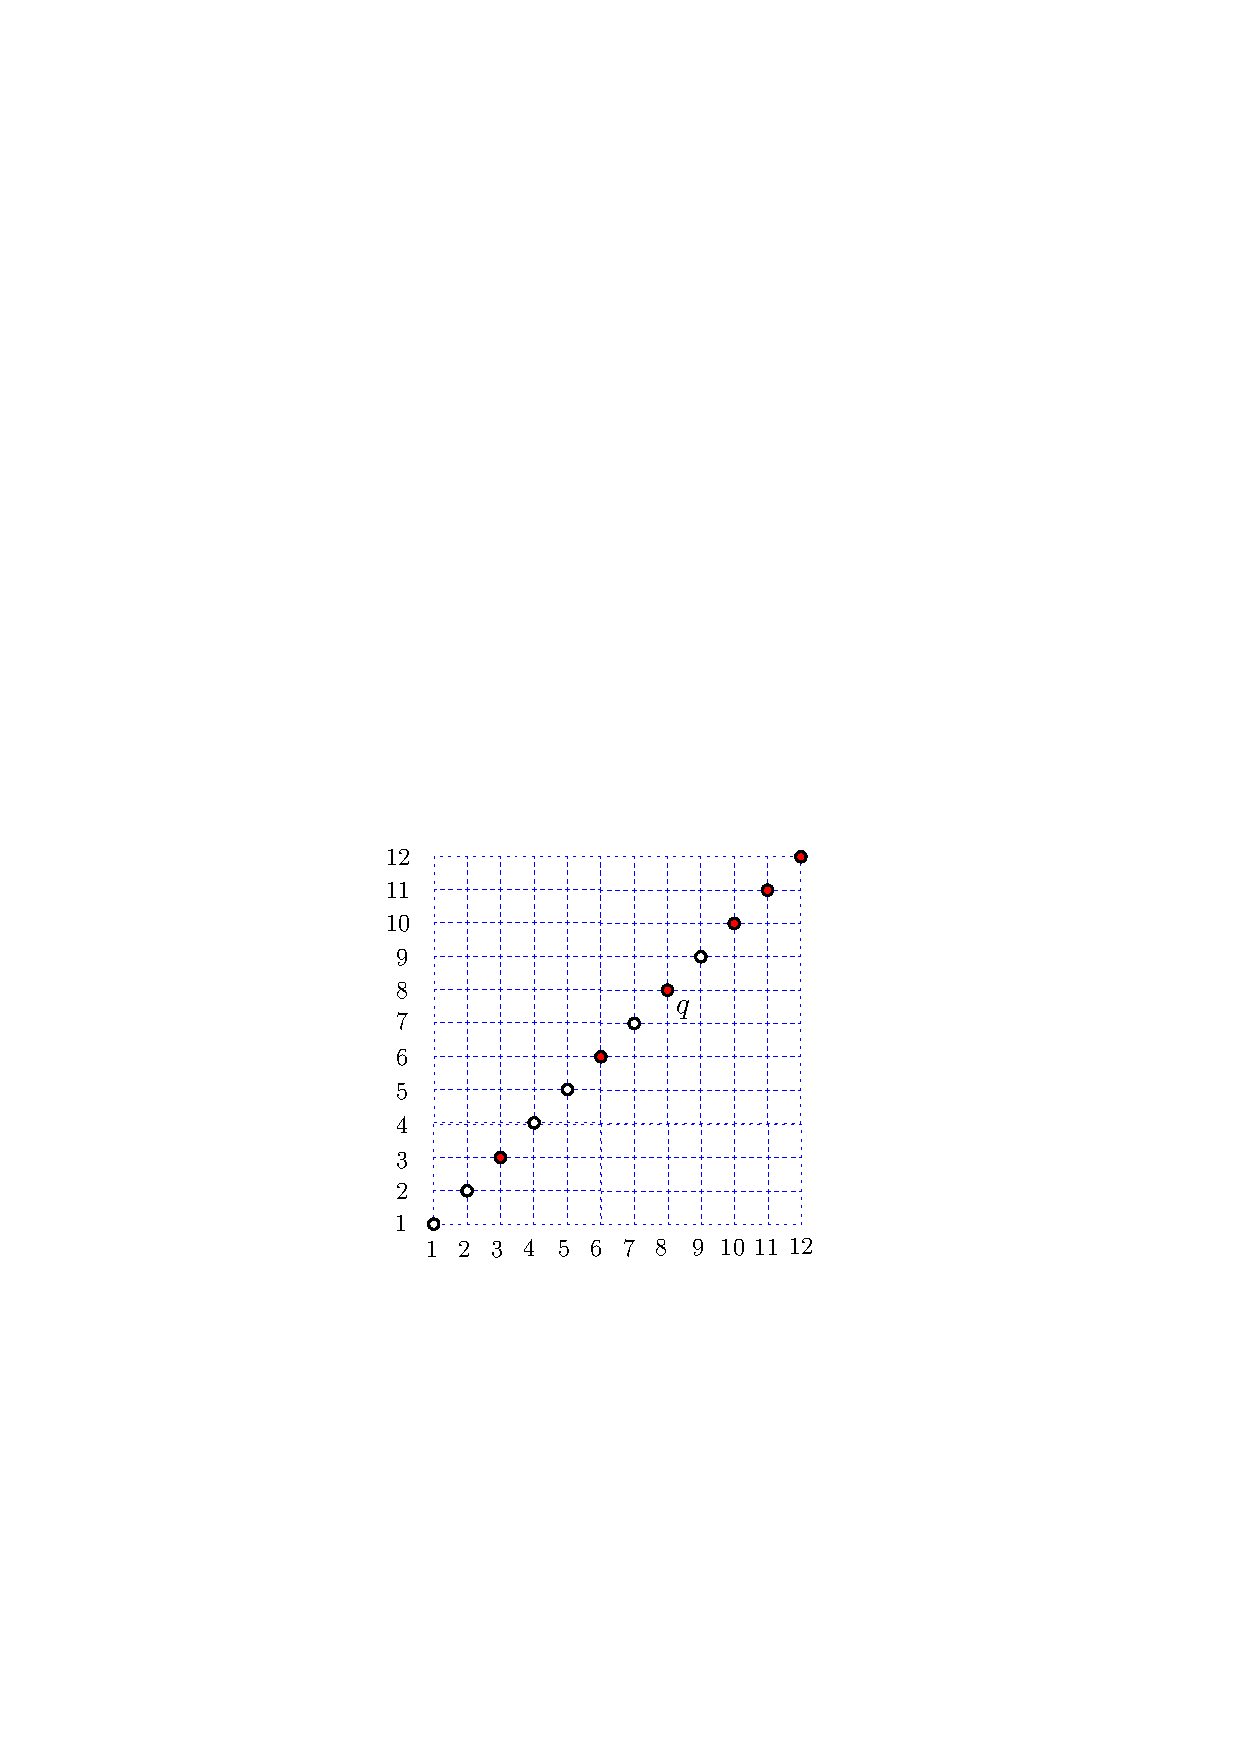
\includegraphics[height=50mm]{./artwork/noisy-ds}
\end{center}

\begin{itemize}
    \item What is the width of the dataset? 
    \item What is the value of $k$? Recall that $k$ is the smallest error of a monotone classifier.
\end{itemize}


\begin{sol}
\extraspacing {\bf Answer:} The width is 1, and $k$ = 3.
\end{sol}


\extraspacing {\bf Problem 2.} Prove: the fractional edge covering number of a triangle must be at least 1.5. 

\begin{sol}
\extraspacing {\bf Answer:} Let $A, B, C$ be the three vertices of a triangle, and let $w_A, w_B$, $w_C$ be their weights, respectively. We know: 
\myeqn{
    w_A + w_B &\ge& 1.5 \nn \\
    w_B + w_C &\ge& 1.5 \nn \\
    w_A + w_C &\ge& 1.5. \nn  
}
Hence: 
\myeqn{
    2(w_A + w_B + w_C) &\ge& 3 \nn  
}
which means that $w_A + w_B + w_C$ must be at least 1.5. 
\end{sol}

\extraspacing {\bf Problem 3.} Prove: a graph $G$ with $m$ edges can contain $O(m^{1.5})$ triangles. 

\begin{sol}
\extraspacing {\bf Answer:} Call a vertex of $G$ {\em small} if its degree is at most $\sqrt{m}$; otherwise, call it {\em large}. The number of large vertices is at most $2m / \sqrt{m} = 2\sqrt{m}$. We divide the triangles into two types: 
\myenums{
    \item At least one vertex $u$ is small, whereas the other vertices $v$ and $w$ can be small or large. There are at most $m^{1.5}$ triangles of this type. First, choose an edge $\set{u,v}$ with (at least) one small vertex $u$; there are $m$ ways to do so. For each $\set{u, v}$, there are at most $\sqrt{m}$ choices of $w$ because $u$ has at most $\sqrt{m}$ neighbors.
    
    \item All vertices are large. The number of triangles of this type is clearly $(2\sqrt{m})^3 = 8m^{1.5}$.
}
\end{sol}


%\bibliographystyle{abbrv}
%\bibliography{../ref}

\end{document}
